% THGEM anode signal study -- short talk (main ~13 min) + backup
% Content: THGEM_anode_signal_report_2026-11-11.pdf (no new simulations).
% Build: pdflatex thgem_anode_signal_talk.tex  (run twice for links)
\documentclass[aspectratio=169,11pt]{beamer}

\usepackage[T1]{fontenc}
\usepackage[utf8]{inputenc}
\usepackage{lmodern}
\usepackage{textcomp}
\usepackage{booktabs}
\usepackage{array}
\newcolumntype{L}[1]{>{\raggedright\arraybackslash}p{#1}}
\usepackage{siunitx}
\sisetup{detect-all, range-phrase=--, range-units=single}
\usepackage{appendixnumberbeamer}
\usepackage{tikz}

% ---------- look ----------
\usetheme{default}
\definecolor{ink}{HTML}{1F2933}
\definecolor{accent}{HTML}{2A6FDB}   % sim blue (matches figures)
\definecolor{lab}{HTML}{E8663D}      % lab orange (matches figures)
\definecolor{warn}{HTML}{B4232A}
\definecolor{muted}{HTML}{6B7280}
\definecolor{boxbg}{HTML}{EEF3FB}
\definecolor{backbg}{HTML}{F5F5F5}
\setbeamercolor{normal text}{fg=ink}
\setbeamercolor{frametitle}{fg=ink}
\setbeamercolor{title}{fg=ink}
\setbeamercolor{structure}{fg=accent}
\setbeamercolor{alerted text}{fg=warn}
\setbeamercolor{button}{bg=accent!15,fg=accent!80!black}
\setbeamerfont{frametitle}{series=\bfseries,size=\Large}
\setbeamertemplate{navigation symbols}{}
\setbeamertemplate{itemize items}[circle]
\newif\ifbackup
\setbeamertemplate{footline}{%
  \leavevmode\hbox to \paperwidth{\hfill\color{muted}\scriptsize
  \ifbackup B\fi\insertframenumber\hspace*{1em}}\vskip3pt}
\setlength{\leftmargini}{1.2em}

% ---------- helpers ----------
% link from a main slide to a backup slide
\newcommand{\bk}[2]{\hyperlink{#1}{\beamergotobutton{#2}}}
% link from a backup slide back to the main slide that uses it
\newcommand{\backlink}[1]{\hfill\hyperlink{#1}{\beamerreturnbutton{back}}}
\newcommand{\labv}[1]{{\color{lab}\textbf{#1}}}
\newcommand{\simv}[1]{{\color{accent}\textbf{#1}}}
\newcommand{\caveat}[1]{{\small\color{warn}\textbf{Caveat:} #1}}
\newcommand{\src}[1]{{\scriptsize\color{muted}#1}}
\newcommand{\Rglass}{R_\text{glass}}
\newcommand{\RCu}{R_\text{Cu}}
\newcommand{\Qtop}{Q_\text{top}}
\newcommand{\Eind}{E_\text{ind}}
\newcommand{\er}{\varepsilon_r}
\newcommand{\takeaway}[1]{%
  \vspace{4pt}\colorbox{boxbg}{\parbox{\dimexpr\linewidth-2\fboxsep}{\small #1}}}

\title{Why the THGEM anode signal shrinks at small induction gaps}
\subtitle{Garfield++ simulation vs measurement: resistive-glass anode}
\author{Luca}
\date{Study status of 11 November 2026; lab data updated 22 November 2026}
\institute{Code, docs and data: \href{https://github.com/lmoleri/THGEM-garfield}{\texttt{github.com/lmoleri/THGEM-garfield}}}

\begin{document}

% ======================================================================
\begin{frame}[plain]
  \titlepage
  \vspace{-1.5em}
  \begin{center}\src{Simulation numbers from the study report of 11 Nov 2026
  (repo \texttt{lmoleri/THGEM-garfield}, commit \texttt{d431c49}); no new simulations.\\
  Lab numbers: exact values from the original plots (22 Nov); sims compared with the $E_\text{ind}$ = 1.5\,kV/cm series.\\
  Colour code in all plots: \labv{orange = lab}, \simv{blue = simulation}.}\end{center}
\end{frame}

% ======================================================================
\begin{frame}[label=m-obs]{The observation: $R = Q_\text{anode}/\Qtop$ drops at small gaps}
  \centering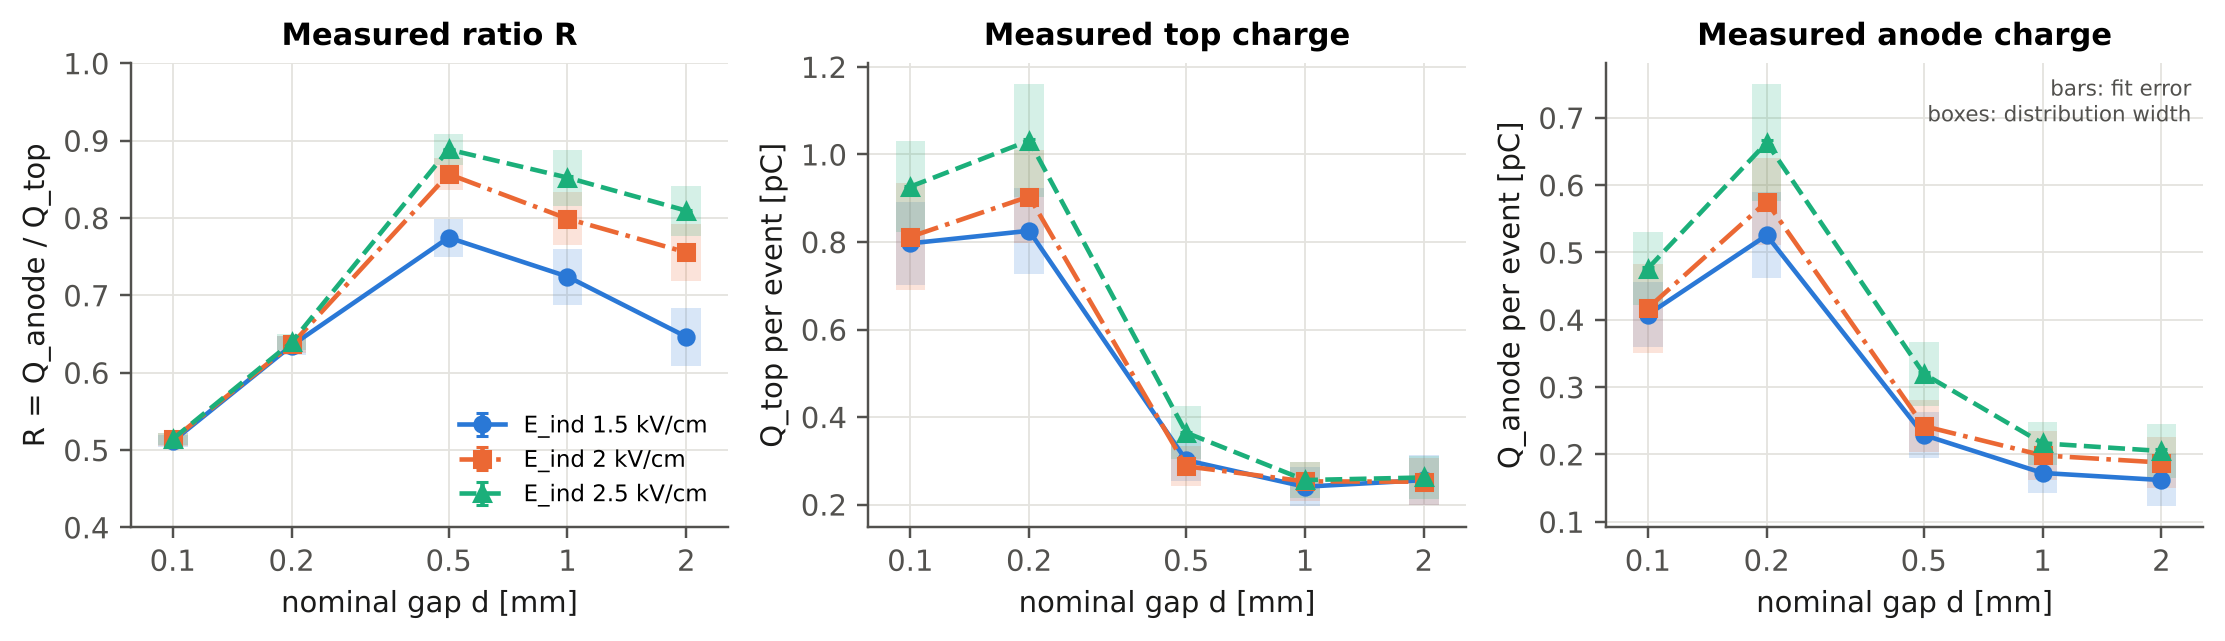
\includegraphics[width=\linewidth]{fig/fig_measured_v2.png}\\[-2pt]
  \raggedright\small
  \begin{columns}[T]
    \begin{column}{0.5\textwidth}
      \begin{itemize}
        \item $R(\Eind{=}1.5)$ = \labv{0.51 / 0.64 / 0.77 / 0.72 / 0.65} at $d$ = 0.1 / 0.2 / 0.5 / 1 / 2\,mm
        \item At 0.1--0.2\,mm $R$ is the same for all three fields (within 0.005) $\Rightarrow$ small-gap suppression is \textbf{field-independent}
      \end{itemize}
    \end{column}
    \begin{column}{0.5\textwidth}
      \begin{itemize}
        \item At $\ge$0.5\,mm $R$ \textbf{rises with field} (0.77$\to$0.89 at 0.5\,mm), via the anode charge
        \item $\Qtop$ rises 3--4$\times$ below 0.5\,mm
      \end{itemize}
      \src{Bars: fit errors; boxes: distribution widths.}\ \bk{b-data}{B1}
    \end{column}
  \end{columns}
\end{frame}

% ======================================================================
\begin{frame}[label=m-det]{Detector, and why the gap convention matters}
  \begin{columns}[T]
    \begin{column}{0.52\textwidth}
      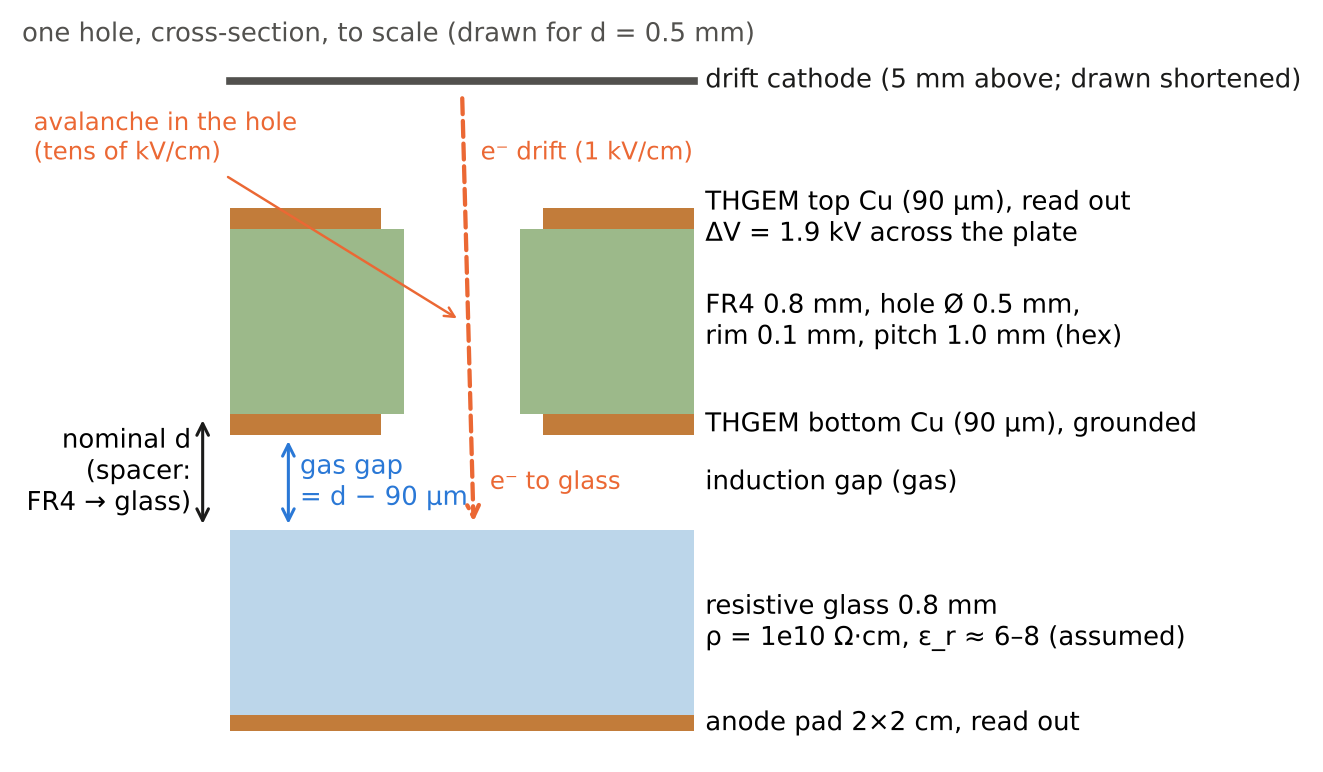
\includegraphics[width=\linewidth]{fig/fig_geometry.png}
    \end{column}
    \begin{column}{0.48\textwidth}
      \small
      \begin{itemize}
        \item THGEM: FR4 0.8\,mm, Cu \SI{90}{\micro m} both faces, hole \O\,0.5\,mm, pitch 1\,mm, \textbf{hexagonal} (sim: square), $\Delta V$ = 1.9\,kV
        \item Ar/CO$_2$ 93:7, $^{55}$Fe, drift 5\,mm at 1\,kV/cm
        \item Anode = 2$\times$2\,cm pad \textbf{behind 0.8\,mm resistive glass} ($\rho = 10^{10}\,\Omega\,$cm)
        \item Spacers set $d$ from the \emph{FR4}: \textbf{gas gap = $d - \SI{90}{\micro m}$}
      \end{itemize}
      \vspace{2pt}
      \centering\footnotesize
      \begin{tabular}{lcccc}\toprule
        nominal $d$ [mm] & 0.1 & 0.2 & 0.5 & 1.0\\
        gas gap [\si{\micro m}] & \textbf{10} & 110 & 410 & 910\\
        gas field [kV/cm] & \textbf{15} & 2.7 & 1.8 & 1.65\\\bottomrule
      \end{tabular}\\[4pt]
      \raggedright\bk{b-det}{B2 parameters}\ \bk{b-history}{B21 how we got here}
    \end{column}
  \end{columns}
  \takeaway{The 10\,\si{\micro m} gas gap at nominal 0.1\,mm (field $\approx$ hole field) is mechanically demanding over 2$\times$2\,cm. Correction found only on 10 Nov; it changed the picture.}
\end{frame}

% ======================================================================
\begin{frame}[label=m-glass]{Key physics: the pad sees electrons on the glass only partially}
  \centering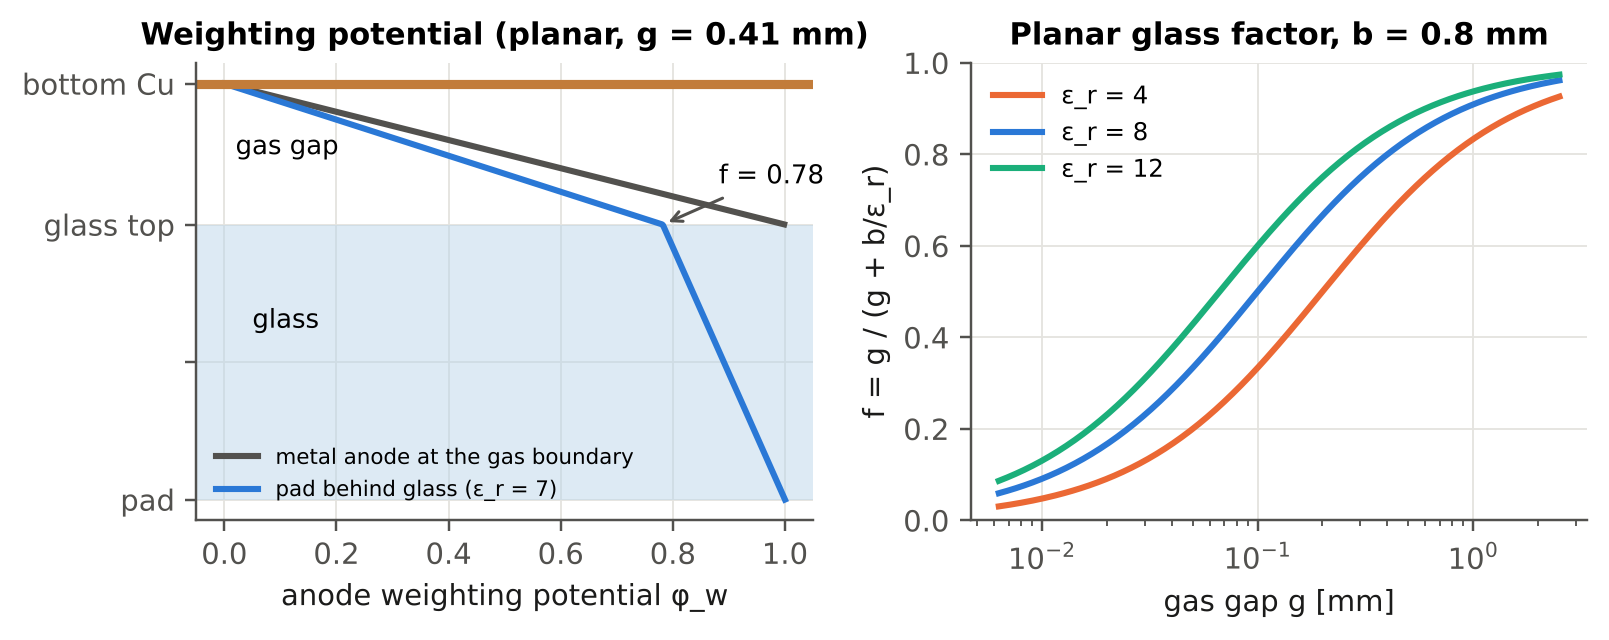
\includegraphics[width=0.70\linewidth]{fig/fig_weighting.png}\\[-2pt]
  \raggedright\small
  \begin{columns}[T]
    \begin{column}{0.5\textwidth}
      \begin{itemize}
        \item Signals are \textbf{induced} (Shockley--Ramo), $Q_k = \sum_i q_i\,\varphi_k(\mathbf{x}_i)$
        \item Electrons stop on the \textbf{glass surface}; glass relaxes in $\tau\approx$ 8--80\,ms $\gg$ readout $\Rightarrow$ a \textbf{dielectric} for the signal
      \end{itemize}
    \end{column}
    \begin{column}{0.5\textwidth}
      \begin{itemize}
        \item Planar factor $f = g/(g + b/\er)$; glass acts like an extra gap $b/\er\approx$ 0.10--0.13\,mm. The rest appears on the THGEM \textbf{bottom}
      \end{itemize}
      \src{Analytic planar curves, not simulation.}\ \bk{b-sr}{B3}\ \bk{b-tau}{B4}\ \bk{b-csa}{B5}
    \end{column}
  \end{columns}
\end{frame}

% ======================================================================
\begin{frame}[label=m-sim]{Simulation chain}
  \small
  \begin{columns}[T]
    \begin{column}{0.5\textwidth}
      \textbf{Transport} (Garfield++, one C++ program)
      \begin{itemize}
        \item Field: \textbf{neBEM} periodic unit cell ($\ge 9$ copies), \textbf{exact} (raw) field; grid interpolation was wrong at the Cu edge (found \& fixed)
        \item Gas: 110-point Magboltz table, Ar/CO$_2$ 93:7, Penning $r = 0.405$ (\emph{assumed})
        \item Avalanche: \textbf{weighted mean-avalanche paths} with diffusion; ions drifted too
      \end{itemize}
    \end{column}
    \begin{column}{0.5\textwidth}
      \textbf{Signal: paired copper/glass replay}
      \begin{itemize}
        \item Snapshot of all charges at 5/10/20\,\si{\micro s}
        \item Score the \emph{same} snapshot with copper-anode and glass-anode weighting potentials ($\er$ 4--12)
        \item $F = \Rglass/\RCu$ is \textbf{paired}: $\pm 0.002$, vs $\pm 5\%$ on $R$
        \item Checks: charge conservation $\le 5\times10^{-15}$, $\sum\varphi_k = 1$, planar-glass benchmark $<0.001\%$
      \end{itemize}
    \end{column}
  \end{columns}
  \vspace{4pt}
  \caveat{transport uses the \emph{metal}-anode field; weights are heavy-tailed (ESS 74--189 of 500 for $\Qtop$), so $\pm$6--10\% bootstrap errors may be optimistic. Quick test: 5$\times$100 paths/gap, one $\Eind$ (1.5).}\\[3pt]
  \bk{b-grid}{B6 grid artefact}\ \bk{b-ess}{B7 weighted paths \& ESS}\ \bk{b-replay}{B8 replay \& validation}
\end{frame}

% ======================================================================
\begin{frame}[label=m-F]{Result 1: the glass factor $F$ has the right shape}
  \begin{columns}[T]
    \begin{column}{0.48\textwidth}
      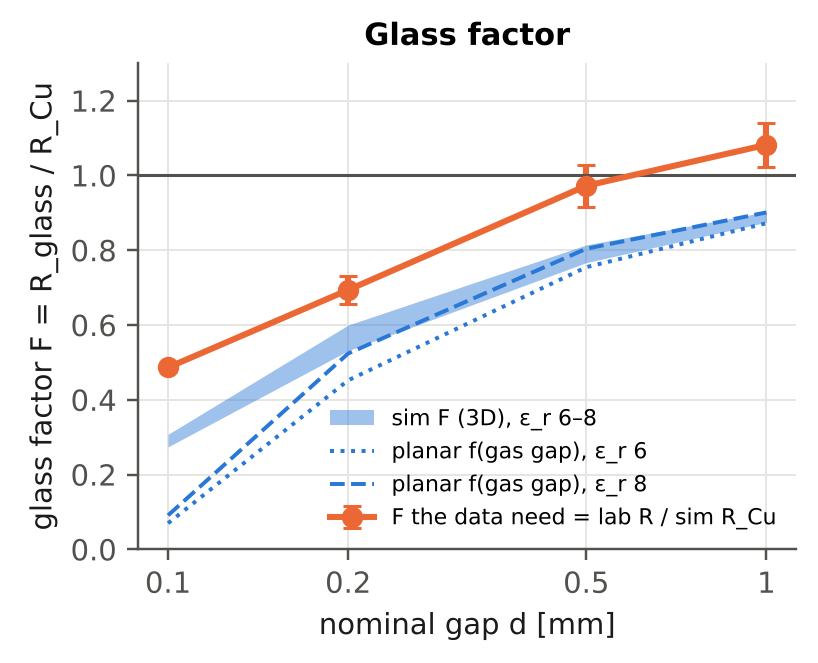
\includegraphics[width=\linewidth]{fig/fig_ratio_v2_R.png}
    \end{column}
    \begin{column}{0.52\textwidth}
      \small
      \begin{itemize}
        \item Simulated 3D $F = \Rglass/\RCu$ ($\er$ 6--8):\\ \simv{0.27--0.31 / 0.53--0.60 / 0.77--0.81 / 0.88--0.90}
        \item $\approx 0.9$ at 1\,mm, steep fall below 0.5\,mm; pure electrostatics $\Rightarrow$ field-independent, as the data are at 0.1--0.2\,mm
        \item At 0.1\,mm 3D $F \gg$ planar $f$ (0.07--0.09): the avalanche starts \emph{inside} the hole
        \item Only mechanism found that lowers $R$ in the observed direction
        \item Orange curve: see next two slides
      \end{itemize}
      \caveat{$\er$ is assumed: $F$(0.2\,mm) = 0.43 / 0.60 / 0.69 at $\er$ = 4 / 8 / 12.}\\[3pt]
      \bk{b-planar}{B9 3D vs planar}\ \bk{b-table}{B10 full table}
    \end{column}
  \end{columns}
\end{frame}

% ======================================================================
\begin{frame}[label=m-cu]{Result 2: but the simulated copper baseline \emph{falls} with the gap}
  \centering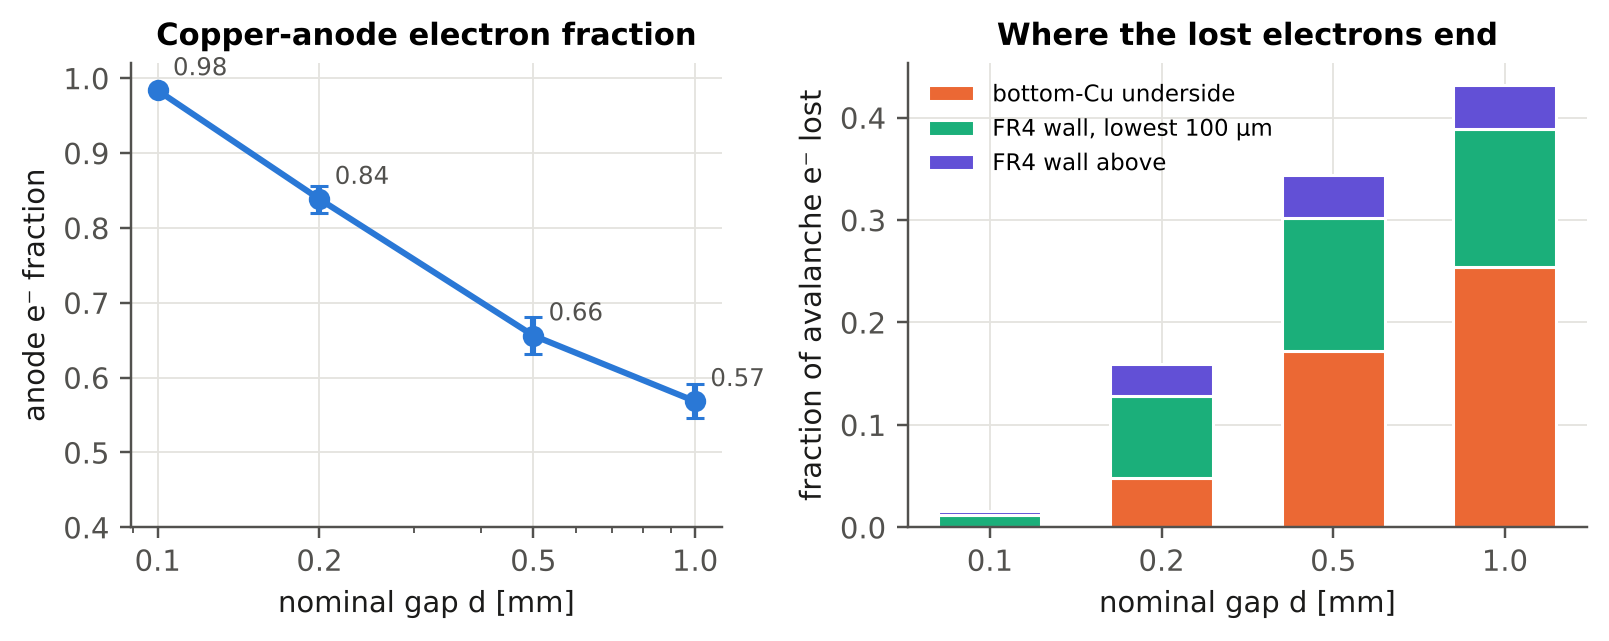
\includegraphics[width=0.74\linewidth]{fig/fig_copper.png}\\[-2pt]
  \raggedright\small
  \begin{columns}[T]
    \begin{column}{0.5\textwidth}
      \begin{itemize}
        \item Copper-anode e$^-$ fraction \simv{0.98 / 0.84 / 0.66 / 0.57}
        \item Lost mostly on the \textbf{underside of the bottom Cu} (25\% at 1\,mm) and the lowest \SI{100}{\micro m} of the FR4 wall (8--14\%)
      \end{itemize}
    \end{column}
    \begin{column}{0.5\textwidth}
      \begin{itemize}
        \item Field lines from the hole exit curl back onto the bottom Cu as the gap grows (\emph{inferred})
        \item \textbf{Not} a gain effect: same fall at $\sim$10$\times$ lower gain\ \bk{b-gainmatched}{B11}
      \end{itemize}
    \end{column}
  \end{columns}
\end{frame}

% ======================================================================
\begin{frame}[label=m-R]{Result 3: full model vs data, $\Rglass = F\times\RCu$}
  \begin{columns}[T]
    \begin{column}{0.48\textwidth}
      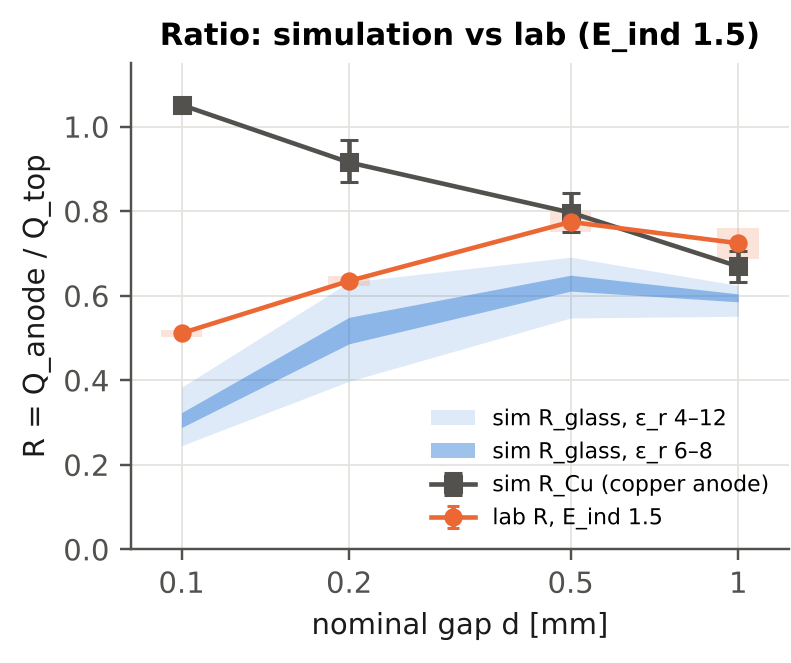
\includegraphics[width=\linewidth]{fig/fig_ratio_v2_L.png}
    \end{column}
    \begin{column}{0.52\textwidth}
      \small
      \begin{itemize}
        \item $\RCu$ falls (1.05 $\to$ 0.67) $\Rightarrow$ $\Rglass$ nearly \textbf{flat} (0.5--0.65), \textbf{0.09--0.16 below} the data at 0.2--1\,mm (0.19--0.22 at 0.1\,mm)
        \item $F$ the data need, lab $R$/sim $\RCu$:\\ \labv{0.49 / 0.69$\pm$0.04 / 0.97$\pm$0.06 / 1.08$\pm$0.06}
        \item At 0.5--1\,mm the data look like a copper anode with \textbf{no glass loss}; glass gives at most 0.87 / 0.93 ($\er$ 12)
        \item[$\Rightarrow$] main remaining error on the \textbf{copper / transport side} (as is the field dependence of lab $R$ at $\ge$0.5\,mm)
      \end{itemize}
      \src{Lab and sim at $\Eind$ 1.5. $\pm$: sim $\RCu$ bootstrap + lab fit error.}\ \bk{b-data}{B1}\ \bk{b-table}{B10}
    \end{column}
  \end{columns}
\end{frame}

% ======================================================================
\begin{frame}[label=m-Q]{Result 4: absolute charges; 0.1\,mm is a clear miss}
  \centering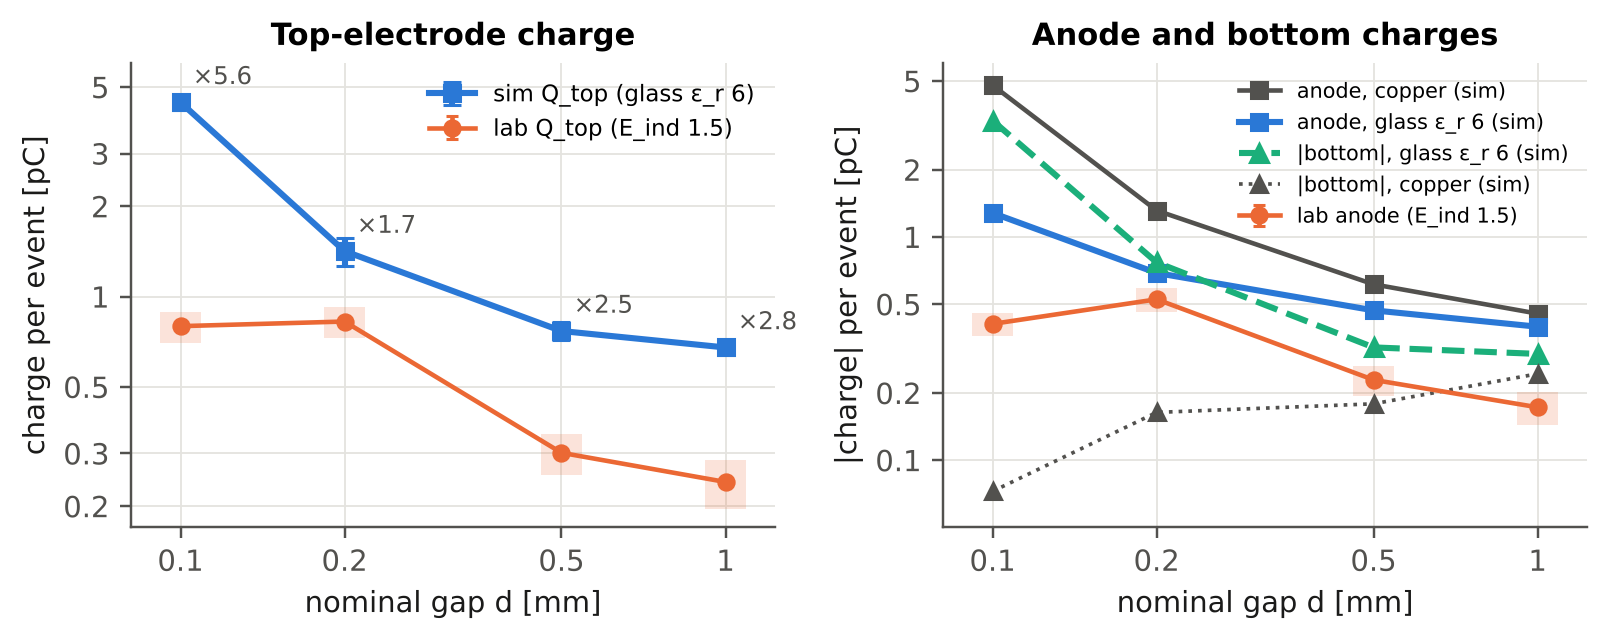
\includegraphics[width=0.74\linewidth]{fig/fig_charges_v2.png}\\[-2pt]
  \raggedright\small
  \begin{columns}[T]
    \begin{column}{0.5\textwidth}
      \begin{itemize}
        \item $\Qtop$ \textbf{shape} data-like at 0.2--1\,mm (0.2/0.5 ratio 1.86 vs lab 2.7)
        \item \textbf{Scale} 1.7--2.8$\times$ high $\approx$ 25--30\,V too much on the THGEM (\emph{inferred}); measured anode charge: sim 1.3--2.3$\times$ high
      \end{itemize}
    \end{column}
    \begin{column}{0.5\textwidth}
      \begin{itemize}
        \item \textbf{0.1\,mm}: gain $1.3\times10^5$, $\Qtop$ \textbf{5.6$\times$} lab
        \item Charge missing at the anode reappears on the \textbf{bottom} (green)
      \end{itemize}
      \caveat{the real 0.1\,mm gap is very likely not a uniform \SI{10}{\micro m}; not modelled.}
    \end{column}
  \end{columns}
\end{frame}

% ======================================================================
\begin{frame}[label=m-ruled]{What has been ruled out (as cause of the gap dependence)}
  \small
  \begin{columns}[T]
    \begin{column}{0.5\textwidth}
      \textbf{Firm}
      \begin{itemize}
        \item Transport-grid artefact at Cu edge (real bug, fixed)
        \item Field mesh (1--2\%; $\le$3.3\% in 10\,\si{\micro m} gap), drift-gap length
        \item Attachment, avalanche space charge, ions reaching anode
        \item Mean-avalanche approximation (microscopic check)
        \item Gain level (gain-matched run)
      \end{itemize}
    \end{column}
    \begin{column}{0.5\textwidth}
      \textbf{Moderate} (assumption-dependent)
      \begin{itemize}
        \item Cu-corner rounding: only 0--45\,\si{\micro m}, old geometry
        \item FR4 charging-up: iterative \& fully-charged limit (square lattice, uniform zones)
        \item Readout impedance: $\le$1.3\% (from the manual, not measured)
        \item Glass surface charging at $\rho = 10^{10}\,\Omega\,$cm: $\approx$0.3\,V vs 15\,V (holds if spot $\gtrsim$1\,mm$^2$)
      \end{itemize}
    \end{column}
  \end{columns}
  \vspace{4pt}
  \bk{b-ruled1}{B12--13 full table}\ \bk{b-imp}{B14 impedance}\ \bk{b-surf}{B15 surface charging}\ \bk{b-fr4}{B16 FR4 charging}
  \takeaway{Several ``moderate'' exclusions were made on the \textbf{square} lattice. If the hexagonal lattice matters, they deserve a second look.}
\end{frame}

% ======================================================================
\begin{frame}[label=m-limits]{Uncertainties and limitations (please read the numbers with these)}
  \footnotesize
  \begin{columns}[T]
    \begin{column}{0.5\textwidth}
      \textbf{Lab side}
      \begin{itemize}
        \item Fit errors are small (R $\le$0.2\%); distribution widths 1.5--6\% (R), 11--24\% (charges). No systematic (calibration) uncertainty given
        \item Gap flatness not measured (0.1\,mm most exposed)
        \item Glass $\er$ and rear contact not measured
      \end{itemize}
      \textbf{Resolved since the report (22 Nov)}
      \begin{itemize}
        \item exact values for all three $\Eind$ series (no more read-off approximations)
        \item old ``lab $R$'' was the $\Eind$ 2.0 series; sims are now compared with the 1.5 series
      \end{itemize}
    \end{column}
    \begin{column}{0.5\textwidth}
      \textbf{Simulation side}
      \begin{itemize}
        \item \textbf{Square} lattice (real: hex); sharp Cu corners; uniform gap
        \item Uncharged FR4/glass; Penning 0.405 assumed; metal-anode transport field
        \item Scored at 10\,\si{\micro s}, not convolved with the 100\,\si{\micro s} CSA decay ($F$ stable 5--20\,\si{\micro s}; $\RCu$, $\Qtop$ not checked)
        \item Heavy-tailed weights: errors may be understated
        \item Quick test only (5$\times$100 paths/gap), \textbf{one $\Eind$ (1.5)}, four gaps: the field dependence at $\ge$0.5\,mm is not simulated
        \item Provenance gaps (unversioned copper-baseline binary, gitignored drivers)
      \end{itemize}
    \end{column}
  \end{columns}
  \bk{b-limits}{B17 details}
\end{frame}

% ======================================================================
\begin{frame}[label=m-next]{Open questions and the most informative next steps}
  \small
  \begin{columns}[T]
    \begin{column}{0.48\textwidth}
      \textbf{Open (ranked by possible weight, \emph{inferred})}
      \begin{enumerate}
        \item Why $\RCu$ falls (0.98$\to$0.57): \textbf{hex lattice} (untested; proxy prepared), real hole-exit profile
        \item Field dependence of $R$ at $\ge$0.5\,mm: run the sim at $\Eind$ 2.0 and 2.5
        \item What the real 0.1\,mm gap looks like
        \item Absolute gain $\sim$2$\times$ high: Penning, gas table, lattice
        \item Glass $\er$ (sets $F$ directly)
        \item Readout time window (10 vs 100\,\si{\micro s})
      \end{enumerate}
      \bk{b-open}{B18 details}
    \end{column}
    \begin{column}{0.52\textwidth}
      \textbf{Lab tests, cheapest first}
      \begin{enumerate}
        \item \textbf{Test pulse} into anode channel at 0.1 and $\ge$1\,mm $\to$ impedance (expect $\le$1.3\% change)
        \item \textbf{Bare copper anode} $\to$ measures $\RCu$ and $F$ directly (sim predicts $\RCu$ 1.05/0.92/0.80/0.67 at $\Eind$ 1.5)
        \item \textbf{Gap \& flatness} at 0.1\,mm
        \item \textbf{Glass $\er$} (capacitance of known area)
        \item Bottom readout at 0.1\,mm ($\sim$3\,pC with glass; can't separate mechanisms)
      \end{enumerate}
      \bk{b-tests}{B19 test table}
    \end{column}
  \end{columns}
\end{frame}

% ======================================================================
\begin{frame}[label=m-summary]{Summary}
  \begin{itemize}
    \item \textbf{Glass anode} is the leading explanation of the small-gap suppression: the pad sees only a fraction $F$ of the electrons stopped on the glass; $F$ is geometric, field-independent, and falls steeply below 0.5\,mm.
    \item \textbf{The full simulation does not yet reproduce the data} (compared at $\Eind$ = 1.5):
      \begin{itemize}
        \item simulated copper baseline falls with gap $\Rightarrow$ $\Rglass$ flat and 0.09--0.16 low at 0.2--1\,mm; data need $F\approx1$ (0.97, 1.08) at 0.5--1\,mm
        \item lab $R$ rises with $\Eind$ at $\ge$0.5\,mm: a transport effect, not glass
        \item $\Qtop$ right shape, 1.7--2.8$\times$ too high; 0.1\,mm a clear miss (real gap probably not a uniform 10\,\si{\micro m})
      \end{itemize}
    \item Many mechanisms ruled out; biggest untested sim candidate: \textbf{hexagonal lattice}.
    \item Cheapest decisive lab inputs: \textbf{test pulse}, \textbf{bare Cu anode}, \textbf{0.1\,mm gap}, \textbf{glass $\er$}.
  \end{itemize}
  \takeaway{Design note (\emph{inferred}): keep $g \gg b/\er$ (thinner / higher-$\er$ glass, or gap $\gtrsim$0.5\,mm) to keep $F\gtrsim0.8$ and make the anode signal insensitive to gap variations.\ \bk{b-ahead}{B20 looking ahead}}
\end{frame}

% ======================================================================
% BACKUP
% ======================================================================
\appendix
\backuptrue
\begin{frame}[plain,noframenumbering]
  \centering\vfill{\Huge\bfseries Backup}\vfill
  \small
  \begin{tabular}{@{}ll@{\hspace{2em}}ll@{}}
    \hyperlink{b-data}{B1} & Lab data (all $\Eind$) & \hyperlink{b-planar}{B9} & 3D $F$ vs planar $f$\\
    \hyperlink{b-det}{B2} & Detector parameters & \hyperlink{b-table}{B10} & Full results table\\
    \hyperlink{b-sr}{B3} & Shockley--Ramo, inventory form & \hyperlink{b-gainmatched}{B11} & Copper baseline, gain-matched\\
    \hyperlink{b-tau}{B4} & Glass as dielectric, $\tau$, $f$ & \hyperlink{b-ruled1}{B12--13} & Ruled-out table\\
    \hyperlink{b-csa}{B5} & Readout timing & \hyperlink{b-imp}{B14} & Readout impedance\\
    \hyperlink{b-grid}{B6} & Grid artefact & \hyperlink{b-surf}{B15} & Glass surface charging\\
    \hyperlink{b-ess}{B7} & Weighted paths \& ESS & \hyperlink{b-fr4}{B16} & FR4 charging-up\\
    \hyperlink{b-replay}{B8} & Paired replay \& validation & \hyperlink{b-limits}{B17} & Limitations in detail\\
     & & \hyperlink{b-open}{B18} & Open questions in detail\\
     & & \hyperlink{b-tests}{B19} & Proposed lab tests\\
     & & \hyperlink{b-ahead}{B20} & Looking ahead\\
     & & \hyperlink{b-history}{B21} & How the study got here\\
     & & \hyperlink{b-prov}{B22} & Data \& provenance\\
     & & \hyperlink{b-refs}{B23} & References\\
  \end{tabular}
  \vfill
\end{frame}

% ---------- B1 ----------
\begin{frame}[label=b-data]{B1 -- Lab data (exact values from the original plots)}
  \centering\scriptsize\renewcommand{\arraystretch}{0.92}
  \begin{tabular}{llccccc}\toprule
    & $\Eind$ [kV/cm] & 0.1 & 0.2 & 0.5 & 1.0 & 2.0\,mm\\\midrule
    $R$ & 1.5 & 0.511 & 0.635 & 0.775 & 0.724 & 0.646\\
        & 2.0 & 0.514 & 0.636 & 0.857 & 0.799 & 0.756\\
        & 2.5 & 0.514 & 0.639 & 0.889 & 0.852 & 0.809\\
    \quad width ($\pm$, 1.5) & & 0.008 & 0.012 & 0.025 & 0.036 & 0.037\\\midrule
    $\Qtop$ [pC] & 1.5 & 0.797 & 0.826 & 0.301 & 0.241 & 0.256\\
        & 2.0 & 0.812 & 0.904 & 0.287 & 0.253 & 0.252\\
        & 2.5 & 0.926 & 1.032 & 0.364 & 0.256 & 0.262\\\midrule
    $Q_\text{anode}$ [pC] & 1.5 & 0.408 & 0.525 & 0.229 & 0.173 & 0.162\\
        & 2.0 & 0.417 & 0.575 & 0.242 & 0.199 & 0.188\\
        & 2.5 & 0.476 & 0.663 & 0.320 & 0.217 & 0.205\\\bottomrule
  \end{tabular}
  \raggedright
  \begin{itemize}\footnotesize\setlength{\itemsep}{0pt}
    \item Extracted from the vector PDFs (\texttt{charge\_ratio}, \texttt{top\_charge}, \texttt{anode\_charge}); extraction error negligible. Fit errors $\le$0.2\% on $R$, $\le$1\% on charges; distribution widths 11--24\% on charges
    \item The report's ``lab $R$'' (0.51/0.64/0.855/0.80/0.755) was the \textbf{2.0} series; its $\Qtop$ was the 1.5 series. Slides now compare the sim (1.5) with the 1.5 series only
    \item $R$ agrees with $Q_\text{anode}/\Qtop$ within $\le$3.4\% (0.5\% at 0.1--0.2\,mm), so $R$ is probably the mean of per-event ratios (\emph{inferred}); the sim forms ratios of pooled charges
  \end{itemize}
  \backlink{m-obs}
\end{frame}

% ---------- B2 ----------
\begin{frame}[label=b-det]{B2 -- Detector and operating parameters}
  \centering\small
  \resizebox{\linewidth}{!}{\begin{tabular}{lll}\toprule
    Item & Value & Status\\\midrule
    THGEM substrate & FR4, 0.8\,mm & lab\\
    Copper & 90\,\si{\micro m} both faces (plate $\approx$0.98\,mm) & lab\\
    Holes & \O\,0.5\,mm, pitch 1.0\,mm, \textbf{hexagonal}, rim 0.1\,mm & lab (\textbf{sim: square})\\
    Active area & $\approx$2$\times$2\,cm (THGEM and pad) & lab\\
    Drift & 5\,mm, 1\,kV/cm & lab\\
    THGEM voltage & $\Delta V$ = 1.9\,kV & lab\\
    Gas & Ar/CO$_2$ 93:7, flowing & lab\\
    Source, rate & $^{55}$Fe 5.9\,keV, $\sim$10\,Hz & lab\\
    Anode & pad behind 0.8\,mm resistive glass, $\rho=10^{10}\,\Omega\,$cm & lab\\
    Glass $\er$ & 6--8 used (scanned 4--12) & \textbf{assumed}\\
    Glass rear contact & ideal ohmic contact over full area & \textbf{assumed}\\
    Readout & DCB209A on top and anode; $C_\text{in,eff}\approx1.84$\,nF; 100\,\si{\micro s} decay; & lab ($C_\text{in,eff}$\\
     & no shaper; bottom Cu hard-grounded; HV via 40\,M$\Omega$ bias input & from manual)\\\bottomrule
  \end{tabular}}
  \backlink{m-det}
\end{frame}

% ---------- B3 ----------
\begin{frame}[label=b-sr]{B3 -- Signal induction: Shockley--Ramo, inventory form}
  \small
  \begin{itemize}
    \item Weighting potential $\varphi_k$: electrode $k$ at 1\,V, all others at 0, \textbf{no free charges, dielectrics in place}
    \item Current and charge induced by a moving charge $q$:
      \[ I_k(t) = q\,\mathbf{E}_k(\mathbf{x}(t))\cdot\mathbf{v}(t),\qquad Q_k = q\,[\varphi_k(\mathbf{x}_1)-\varphi_k(\mathbf{x}_0)] \]
    \item The \emph{real} field decides where charges go; the \emph{weighting} field decides how much each electrode sees
    \item $\sum_k\varphi_k = 1$ $\Rightarrow$ induced charges sum to zero: charge missing on one electrode appears on another (sim: four electrodes sum to 0 within $3\times10^{-14}$)
    \item e$^-$/ion pairs are created at the same point, so at time $T$:
      \[ Q_k(T) = \sum_i q_i\,\varphi_k(\mathbf{x}_i(T)) \]
      used with a snapshot at $T$ = 10\,\si{\micro s}. Equals collected charge only once everything sits on conductors.
    \item Why the top gives a large signal: slow ions moving up from the bottom of the hole
  \end{itemize}
  \backlink{m-glass}
\end{frame}

% ---------- B4 ----------
\begin{frame}[label=b-tau]{B4 -- Glass as a dielectric on the readout time scale}
  \small
  \begin{columns}[T]
    \begin{column}{0.5\textwidth}
      \textbf{Relaxation time} (planar, Riegler JINST 2016):
      \[ \tau = \rho\,\varepsilon_0\Big(\er + \frac{b}{g}\Big) \]
      $\rho = 10^{10}\,\Omega\,$cm (lab), $\er\approx7$ (assumed), $b$ = 0.8\,mm:
      \begin{itemize}
        \item $\tau\approx 8$\,ms at $g$ = 0.41\,mm
        \item $\tau\approx 80$\,ms at $g$ = 10\,\si{\micro m}
      \end{itemize}
      Both $\gg$ 10--100\,\si{\micro s} $\Rightarrow$ glass = pure dielectric for the signal; weighting potential computed with glass in place.
    \end{column}
    \begin{column}{0.5\textwidth}
      \textbf{Planar glass factor}\\
      $D_n$ continuous: $E_\text{glass} = E_\text{gas}/\er$, and $E_\text{gas}g + E_\text{glass}b = 1$:
      \[ f = E_\text{gas}\,g = \frac{g}{g + b/\er} \]
      \begin{itemize}
        \item electron drifting bottom Cu $\to$ glass gives the pad $-fe$, the bottom Cu $-(1-f)e$
        \item glass $\equiv$ extra gas gap $b/\er$ = 0.10--0.13\,mm ($\er$ 6--8)
        \item over $t\gg\tau$ the pad gets the full $-e$, but the CSA has decayed by then
      \end{itemize}
    \end{column}
  \end{columns}
  \backlink{m-glass}
\end{frame}

% ---------- B5 ----------
\begin{frame}[label=b-csa]{B5 -- What the preamplifier measures (timing)}
  \begin{columns}[T]
    \begin{column}{0.55\textwidth}
      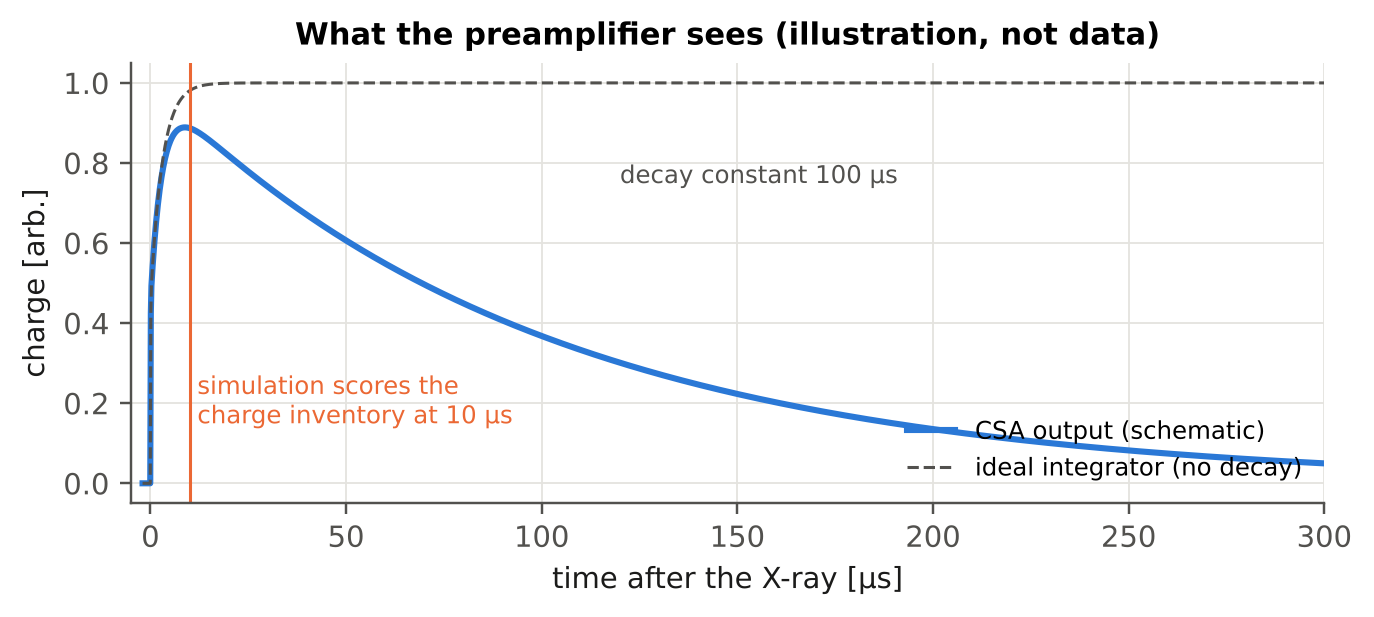
\includegraphics[width=\linewidth]{fig/fig_timeline.png}
      \src{Schematic only: illustrative time constants, not data.}
    \end{column}
    \begin{column}{0.45\textwidth}
      \small
      \begin{itemize}
        \item DCB209A CSA, no shaper, plateau of the digitised pulse, decay 100\,\si{\micro s}
        \item Electron signal: ns. Ions near the hole: \si{\micro s}. Ion drift through the 5\,mm gap: $\sim$370\,\si{\micro s} $>$ decay $\Rightarrow$ partly lost
        \item Simulation scores at \textbf{10\,\si{\micro s}}
        \item $F$ is the same at 5/10/20\,\si{\micro s}; $\RCu$ and $\Qtop$ at the true readout time \textbf{not checked} (open)
      \end{itemize}
    \end{column}
  \end{columns}
  \backlink{m-glass}
\end{frame}

% ---------- B6 ----------
\begin{frame}[label=b-grid]{B6 -- Grid interpolation artefact at the copper edge (fixed)}
  \centering
  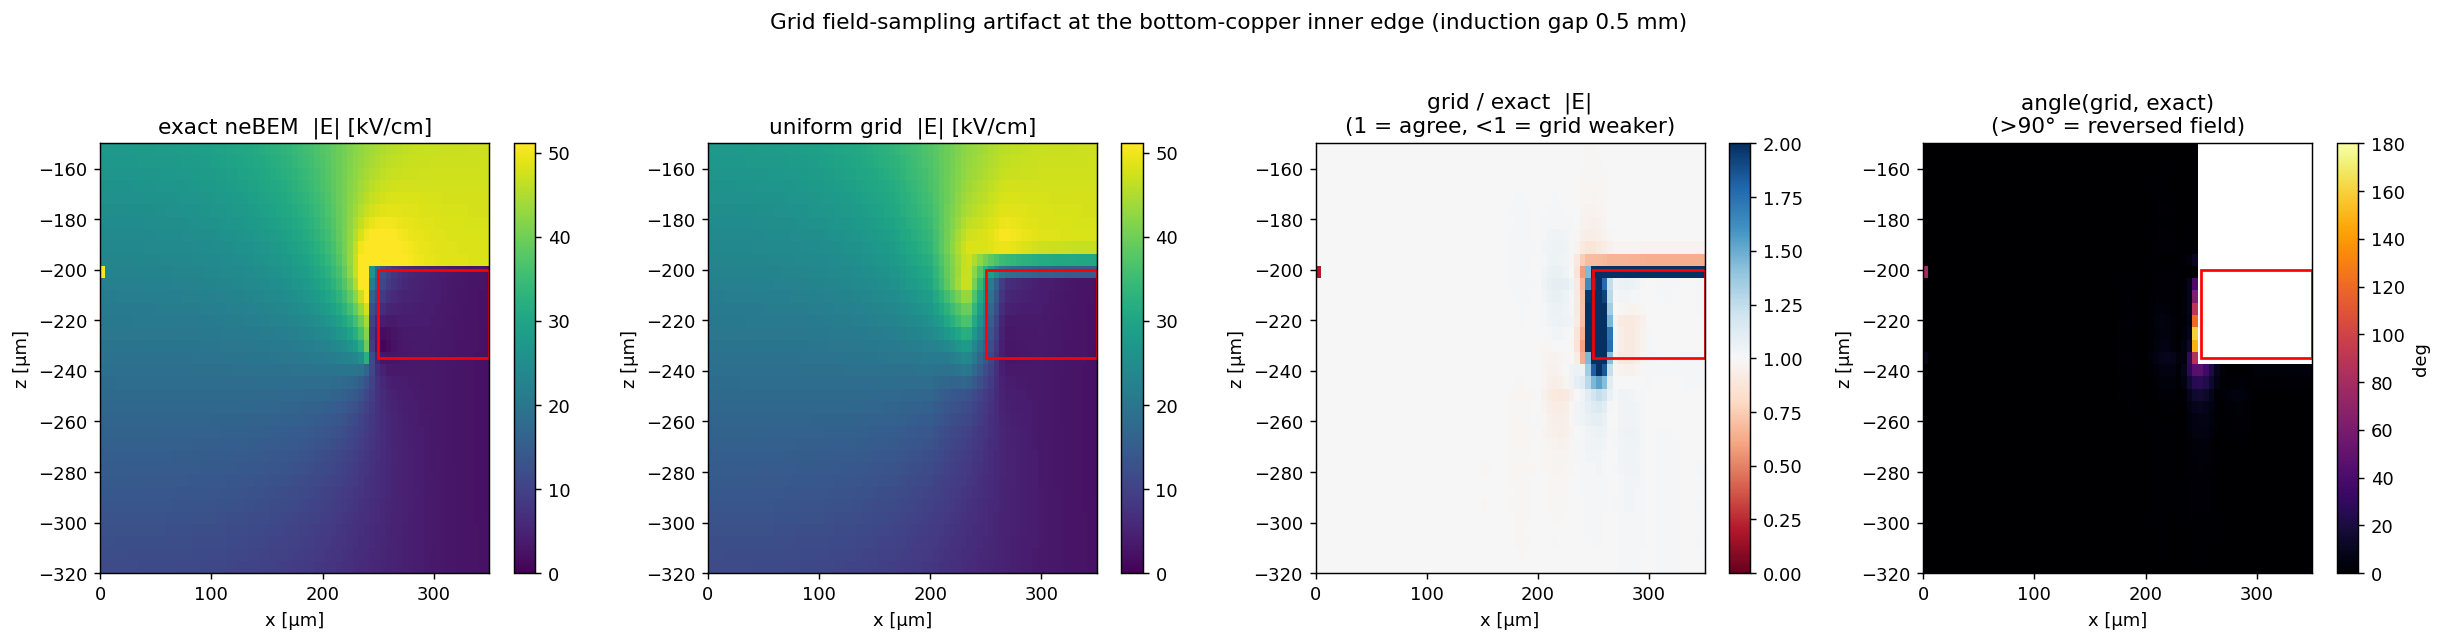
\includegraphics[width=0.95\linewidth]{fig/rawgrid_edge_field.png}
  \raggedright\small
  \begin{itemize}
    \item Old geometry (0.4\,mm plate, 0.5\,mm gap; superseded). Field near the inner edge of the bottom Cu (red outline)
    \item Grid cells straddling Cu and gas mix the gas field with zero field in the metal: wrong by up to 2$\times$, direction reversed in a thin layer $\Rightarrow$ electrons over-extracted
    \item Since then all transport uses the exact (raw) neBEM field. Mesh: 4$\times$ elements changes the field by 1--2\%; 10\,\si{\micro m} gap: 2\,021 vs 13\,938 elements, $\le$3.3\%
  \end{itemize}
  \backlink{m-sim}
\end{frame}

% ---------- B7 ----------
\begin{frame}[label=b-ess]{B7 -- Weighted mean-avalanche paths and effective sample size}
  \small
  \begin{itemize}
    \item At gain $10^4$--$10^5$ microscopic tracking of every electron is too expensive
    \item Representative paths: drift with \texttt{AvalancheMC} (incl.\ diffusion); each path carries a weight $=$ expected number of electrons, from local Townsend $\alpha$ and attachment $\eta$:
      \[ G = \exp\!\Big(\int[\alpha(E)-\eta(E)]\,\mathrm{d}s\Big) \]
      ions created along the path in proportion to the local multiplication, and drifted
    \item Paths through the highest-field region carry very large weights $\Rightarrow$ \textbf{heavy tails}
    \item $\text{ESS} = (\sum w)^2/\sum w^2$: e.g.\ 500 paths with ESS 74 $\approx$ 74 equal paths
      \begin{itemize}
        \item glass $\Qtop$: ESS 74--189 of 500; copper baseline: 455--556 of 1800
        \item bootstrap intervals assume the tail is well sampled $\Rightarrow$ may \textbf{understate} the spread
      \end{itemize}
    \item Microscopic tracking at the hole exit shows the same corner losses $\Rightarrow$ approximation is not the cause
    \item Conventions: 68\% bootstrap; ratios from pooled signed charges; per-event = per-primary $\times$ 227 ($5.9\,\text{keV}/26\,\text{eV}$)
  \end{itemize}
  \backlink{m-sim}
\end{frame}

% ---------- B8 ----------
\begin{frame}[label=b-replay]{B8 -- Paired copper/glass replay and its validation}
  \small
  \begin{enumerate}
    \item \textbf{Export}: transport in the real field with the anode as a metal boundary at the glass surface; snapshot of every charge (e$^-$, ions, attached ions, charges on insulators) at 5, 10, 20\,\si{\micro s}
    \item \textbf{Replay}: score the same snapshot twice: copper-anode weighting potentials, and pad-behind-0.8\,mm-glass at $\er$ = 4--12. Four electrodes: cathode, top, bottom, anode
  \end{enumerate}
  \textbf{Built-in checks}
  \begin{itemize}
    \item charge conservation in every snapshot $\le 5\times10^{-15}$
    \item weighting-potential partition $\sum\varphi_k = 1$, residual $\le 7\times10^{-13}$
    \item all periodic copies evaluated exactly for weighting fields (an approximation for distant copies had caused a 2\% error, fixed)
    \item planar-glass benchmark vs analytic formula: errors $<0.001\%$
    \item regression tests for two trajectory edge cases found in production
  \end{itemize}
  \caveat{transport uses the metal-anode field: charge on the glass or a DC drop across it would change it (argued small, see B15).}
  \backlink{m-sim}
\end{frame}

% ---------- B9 ----------
\begin{frame}[label=b-planar]{B9 -- Why the 3D $F$ exceeds the planar $f$ at 0.1\,mm}
  \small
  \begin{itemize}
    \item Planar $f$ at a 10\,\si{\micro m} gas gap: 0.07--0.09 ($\er$ 6--8). 3D $F$: \textbf{0.27--0.31}
    \item Avalanche electrons start \emph{inside the hole}, where the anode weighting potential is already well above zero: through the holes the weighting field reaches into the THGEM, so the effective gap is larger than the Cu--glass clearance (\emph{inferred})
    \item At 0.5--1\,mm the planar formula is within a few \% of the 3D result
    \item Dependence on the assumed $\er$ (0.2\,mm): $F$ = 0.43 / 0.60 / 0.69 at $\er$ = 4 / 8 / 12. At 0.2\,mm, $\er$ = 12 would match the data ($\Rglass$ 0.63 vs 0.635), but not at 0.5 or 1\,mm
    \item Measured glass $\er$ would remove the main assumed input to $F$
  \end{itemize}
  \vspace{6pt}
  \centering\footnotesize
  \begin{tabular}{lcccc}\toprule
    nominal $d$ [mm] & 0.1 & 0.2 & 0.5 & 1.0\\\midrule
    sim 3D $F$, $\er$ 6--8 & 0.27--0.31 & 0.53--0.60 & 0.77--0.81 & 0.88--0.90\\
    sim 3D $F$, $\er$ 12 & 0.36 & 0.69 & 0.87 & 0.93\\
    $F$ the data need (lab $R$ at 1.5 / sim $\RCu$) & 0.49 & 0.69 & 0.97 & 1.08\\\bottomrule
  \end{tabular}
  \par\raggedright\backlink{m-F}
\end{frame}

% ---------- B10 ----------
\begin{frame}[label=b-table]{B10 -- Real-geometry results (sim $\er$ 6--8; lab $\Eind$ 1.5 in brackets)}
  \centering\footnotesize
  \resizebox{\linewidth}{!}{\begin{tabular}{lcccc}\toprule
    nominal $d$ & 0.1\,mm & 0.2\,mm & 0.5\,mm & 1.0\,mm\\\midrule
    $\Qtop$ [pC] & 4.44--4.47 (\labv{0.80}) & 1.42 (\labv{0.83}) & 0.77 (\labv{0.30}) & 0.68 (\labv{0.24})\\
    $\Qtop$ sim/lab & 5.6 & 1.7 & 2.5 & 2.8\\
    $Q_\text{anode}$ glass $\er$ 6 [pC] & 1.28 (\labv{0.41}) & 0.69 (\labv{0.53}) & 0.47 (\labv{0.23}) & 0.40 (\labv{0.17})\\
    $\Rglass$ & 0.29--0.32 (\labv{0.51}) & 0.49--0.55 (\labv{0.64}) & 0.61--0.65 (\labv{0.77}) & 0.59--0.60 (\labv{0.72})\\
    $\RCu$ & 1.05 & 0.92 & 0.80 & 0.67\\
    $F = \Rglass/\RCu$ & 0.27--0.31 & 0.53--0.60 & 0.77--0.81 & 0.88--0.90\\
    lab $R$ / sim $\RCu$ & 0.49 & 0.69 & 0.97 & 1.08\\
    Cu anode e$^-$ fraction & 0.984 & 0.838 & 0.656 & 0.568\\
    \quad lost on bottom-Cu underside & 0.001 & 0.048 & 0.172 & 0.254\\
    \quad lost on lowest 100\,\si{\micro m} of wall & 0.012 & 0.080 & 0.130 & 0.135\\
    mean gain & $1.3\times10^5$ & $3.6\times10^4$ & $2.4\times10^4$ & $2.2\times10^4$\\
    $|Q_\text{bottom}|$ with glass [pC] & 3.2--3.3 & 0.68--0.77 & 0.29--0.32 & 0.29--0.30\\\bottomrule
  \end{tabular}}\\[6pt]
  \raggedright\small
  Setup: Cu 90\,\si{\micro m}, gas gaps 10/110/410/910\,\si{\micro m} at the fields of the gap table, $\Delta V$ 1.9\,kV, $E_d$ 1\,kV/cm, $\Eind$ 1.5, square lattice, uncharged insulators. Glass signal 5$\times$100 paths/gap at 10\,\si{\micro s}; copper baseline 3$\times$600 paths/gap.\\
  Precision: charges $\pm$6--10\%, $R$ $\pm$5\% ($\pm$1\% at 0.1\,mm), $F$ $\pm$0.002 (paired), Cu fraction $\pm$0.02. \textbf{Heavy tails: see B7.}
  \backlink{m-R}
\end{frame}

% ---------- B11 ----------
\begin{frame}[label=b-gainmatched]{B11 -- The falling copper baseline is geometric, not gain-driven}
  \small
  \begin{itemize}
    \item Mechanism (\emph{inferred}): as the gap grows the induction field weakens relative to the hole field; more field lines from the hole exit curl back to the \textbf{underside of the bottom Cu}
    \item Real geometry, $\Delta V$ 1.9\,kV: anode e$^-$ fraction 0.98 / 0.84 / 0.66 / 0.57; bottom-Cu loss 0.001 / 0.048 / 0.172 / 0.254
    \item \textbf{Gain-matched test} ($\Delta V$ 1.77\,kV, gain $\sim$10$\times$ lower, old Cu 50\,\si{\micro m} geometry): 0.88 / 0.80 / 0.69 at 0.1 / 0.2 / 0.5\,mm $\Rightarrow$ same fall
    \item Field matters for the baseline: at 0.2\,mm the sim Cu fraction rises 0.78 $\to$ 0.88 for $\Eind$ 1 $\to$ 3\,kV/cm (old geometry). In the lab, $R$ at $\ge$0.5\,mm rises $\sim$15\% from $\Eind$ 1.5 to 2.5: qualitatively the same kind of field-dependent extraction (\emph{inferred}, not simulated at the real geometry)
    \item Even a perfect FR4 shield (no wall loss) leaves the bottom-Cu loss, so the baseline would still fall (B16)
  \end{itemize}
  \caveat{gain-matched run was on the old 50\,\si{\micro m} Cu geometry and nominal gaps; the shape argument should carry over, but it was not re-run.}
  \backlink{m-cu}
\end{frame}

% ---------- B12 ----------
\begin{frame}[label=b-ruled1]{B12 -- Ruled out (1/2): firm exclusions}
  \centering\footnotesize
  \begin{tabular}{L{0.24\linewidth}L{0.27\linewidth}L{0.38\linewidth}}\toprule
    Mechanism & Test & Why excluded\\\midrule
    Transport-grid artefact at Cu edge & raw neBEM vs grid; wall-release test & real bug, caused early over-extraction; \textbf{fixed}\\
    Field mesh & elements $\times4$; 10\,\si{\micro m}: 2\,021 vs 13\,938 & field changes 1--2\% ($\le$3.3\% in 10\,\si{\micro m} gap)\\
    Drift gap 1 vs 5\,mm & field comparison & $<1.4\%$ in hole and gap field\\
    Electron attachment & CO$_2$ variation, Magboltz & small and gap-flat\\
    Space charge; ions to anode & self-field estimate; ion field lines incl.\ charged rim & $\sim10^3\times$ too weak; ions reach anode only at 3--10\,pC/event (lab 0.2--0.8) [0.4\,mm plate]\\
    Mean-avalanche approx. & weighted vs microscopic at hole exit & same corner loss\\
    Gain level & gain-matched $\Delta V$ 1.77\,kV & same fall at $\sim10\times$ lower gain\\
    Extraction fraction as observable & ions followed in 3D & wrong observable (top gets only $\sim$45\% of ions); replaced by induced charge\\\bottomrule
  \end{tabular}
  \backlink{m-ruled}\ \hyperlink{b-ruled2}{\beamergotobutton{next: B13}}
\end{frame}

% ---------- B13 ----------
\begin{frame}[label=b-ruled2]{B13 -- Ruled out (2/2): moderate exclusions}
  \centering\footnotesize
  \begin{tabular}{L{0.19\linewidth}L{0.24\linewidth}L{0.29\linewidth}L{0.16\linewidth}}\toprule
    Mechanism & Test & Why excluded & Weak point\\\midrule
    Cu-corner rounding & radius 0--45\,\si{\micro m}, 0.4\,mm plate & only 45\,\si{\micro m} gives a flat trend; all far below data & real radius unknown; old geometry\\
    FR4 charging, iterative & 12 neBEM iterations, 0.1 \& 0.5\,mm & no equilibrium; gain collapses 250--900$\times$; extraction doesn't move toward data & \\
    FR4 charging, fully charged & wall charge for zero normal field, 12 bands + rims, 0.5\,mm & needs 10--20\,nC/cm$^2$ $\to$ hole field $\times$0.4 (no gain); gain allows $\lesssim$1--2\,nC/cm$^2$ & uniform zones, square lattice\\
    Readout impedance & capacitive divider, DCB209A values & $\le$1.3\% loss; data would need $C_\text{in,eff}\approx$30--40\,pF & manual, not measured\\
    Glass surface charging (0.1\,mm) & estimate, $\rho=10^{10}\,\Omega\,$cm & $\bar V = J\rho b\approx0.3$\,V vs 15\,V & spot $\ll$1\,mm$^2$\\\bottomrule
  \end{tabular}
  \backlink{m-ruled}
\end{frame}

% ---------- B14 ----------
\begin{frame}[label=b-imp]{B14 -- Readout impedance}
  \small
  \begin{itemize}
    \item Induced anode current splits between the CSA input and $C_{AB}$ (pad $\leftrightarrow$ grounded bottom Cu). Both capacitive $\Rightarrow$ frequency-independent split:
      \[ \frac{Q_\text{CSA}}{Q} = \frac{C_\text{in,eff}}{C_\text{in,eff} + C_{AB}} \]
    \item $C_\text{in,eff}\approx1.84$\,nF: 2\,nF HV coupling cap in series with 100\,nF and virtual ground $A_0C_f\approx30$\,nF (all from the manual)
    \item $C_{AB}$: a few to a few tens of pF (19--25\,pF at 0.1\,mm with glass) $\Rightarrow$ loss $\le$1.3\% (1--3\% generally)
    \item Losing 40\% would need $C_\text{in,eff}\approx$30--40\,pF: $\sim$50$\times$ worse than specified
  \end{itemize}
  \takeaway{Testable: test pulse into the anode channel with the detector connected, at 0.1 and $\ge$1\,mm. Expect $\le$1.3\% difference if the manual is right; $\sim$40\% if impedance were the cause.}
  \backlink{m-ruled}
\end{frame}

% ---------- B15 ----------
\begin{frame}[label=b-surf]{B15 -- Glass surface charging at 0.1\,mm}
  \small
  \begin{itemize}
    \item Only $\sim$15\,V across the 10\,\si{\micro m} gap: a few volts on the glass would matter
    \item Per event $\sim$1\,pC of electrons on the glass; over $\sim$1\,mm$^2$ and $\sim$0.9\,pF gap capacitance $\Rightarrow$ $\sim$1\,V step, decaying with $\tau\approx80$\,ms
    \item An earlier version used $\tau=\varepsilon_0\er\rho\approx6$\,ms: \textbf{wrong} for a charge facing a thin gap (corrected in the docs)
    \item The exclusion holds for another reason: the \textbf{mean} surface potential is set by the current density alone,
      \[ \bar V = J\rho b \approx 0.3\,\text{V}\quad(0.41\,\text{pC}\times10\,\text{Hz on}\ \ge1\,\text{mm}^2) \]
      independent of $\tau$; $\approx2\%$ of the 15\,V
  \end{itemize}
  \caveat{fails if the irradiated spot is $\ll$1\,mm$^2$ or the rate per spot is much higher than assumed; surface/contact resistance of the glass not known.}
  \backlink{m-ruled}
\end{frame}

% ---------- B16 ----------
\begin{frame}[label=b-fr4]{B16 -- FR4 charging-up}
  \small
  \textbf{Iterative} (12 neBEM iterations at 0.1 and 0.5\,mm)
  \begin{itemize}
    \item no equilibrium reached; gain collapses 250--900$\times$; extraction does not move toward the data
  \end{itemize}
  \textbf{Fully-charged limit} (0.5\,mm; fit of wall charge for zero normal field; 12 wall bands + rims)
  \begin{itemize}
    \item clearing the wall needs \textbf{10--20\,nC/cm$^2$}, which cuts the hole field to $\sim$0.4$\times$ (no gain)
    \item the measured gain allows only $\lesssim$1--2\,nC/cm$^2$ $\Rightarrow$ wall field lowered by only 10--15\%
    \item at 0.5\,mm the end points are FR4 wall 0.21 vs bottom-Cu underside 0.10 (old 50\,\si{\micro m} geometry): even a perfect FR4 shield leaves the bottom-Cu loss, so the baseline still falls
  \end{itemize}
  \caveat{azimuthally uniform charge zones, square lattice, no avalanche run in the charged field.}
  \backlink{m-ruled}
\end{frame}

% ---------- B17 ----------
\begin{frame}[label=b-limits]{B17 -- Uncertainties and limitations in detail}
  \footnotesize
  \begin{columns}[T]
    \begin{column}{0.5\textwidth}
      \textbf{Lab}
      \begin{itemize}
        \item fit errors small; distribution widths given; no systematic (calibration) uncertainty
        \item lab $R$ is probably a mean of per-event ratios, sim $R$ a ratio of pooled charges ($\le$3.4\% difference, B1)
        \item gap flatness over the pad not measured
        \item glass $\er$, rear-contact quality not measured
      \end{itemize}
      \textbf{Report and slides}
      \begin{itemize}
        \item background physics simplified; W-value, drift velocities indicative
        \item references quoted from memory; check before citing
        \item lab-data plots on these slides redrawn 22 Nov from the extracted values; the report itself is updated separately
      \end{itemize}
    \end{column}
    \begin{column}{0.5\textwidth}
      \textbf{Simulation}
      \begin{itemize}
        \item geometry: square lattice, sharp Cu corners, uniform planar gap
        \item physics: uncharged FR4 \& glass; Penning $r=0.405$ assumed; metal-anode transport field; 10\,\si{\micro s} scoring, no CSA convolution
        \item statistics: heavy tails, ESS 74--189/500 for glass $\Qtop$; $F$ robust (paired)
        \item scope: one $\Eind$ (1.5), four gaps, quick test 5$\times$100 paths; gated production study interrupted
        \item provenance: copper-baseline binary (\texttt{../THGEM\_corner}) unversioned; some drivers in gitignored \texttt{results/}; dense gas table not in \texttt{gas/}
      \end{itemize}
    \end{column}
  \end{columns}
  \backlink{m-limits}
\end{frame}

% ---------- B18 ----------
\begin{frame}[label=b-open]{B18 -- Open questions in detail}
  \small
  \begin{enumerate}
    \item \textbf{Falling copper baseline} (0.98 $\to$ 0.57), largest error at 0.2--1\,mm. Untested:
      \begin{itemize}
        \item \textbf{hexagonal lattice}: farthest Cu from a hole 0.58\,mm (hex) vs 0.71\,mm (square). Square-pitch-0.93\,mm proxy with the same hole density prepared (\texttt{results/hex\_proxy\_p093/}), parked. A true hex cell needs a mirror-symmetric $p/2\times(\sqrt3/2)p$ unit cell
        \item real hole-exit profile (Cu etched from 150\,\si{\micro m}; corner radius unknown)
      \end{itemize}
    \item \textbf{Field dependence at $\ge$0.5\,mm}: lab $R$ rises $\sim$15\% from $\Eind$ 1.5 to 2.5; the sim has only 1.5. Runs at 2.0 and 2.5 would test whether the model's extraction has the same field slope
    \item \textbf{Real 0.1\,mm gap}: spacer tolerance, flatness, partial contact would raise the effective gap and lower the gain; not modelled
    \item \textbf{Absolute gain $\sim$2$\times$ high} at 0.2--1\,mm: Penning transfer, gas table, lattice
    \item \textbf{Glass $\er$} assumed; sets $F$ directly
    \item \textbf{Time window}: 10\,\si{\micro s} scoring vs 100\,\si{\micro s} CSA decay; $\RCu$, $\Qtop$ not checked at readout time
  \end{enumerate}
  \backlink{m-next}
\end{frame}

% ---------- B19 ----------
\begin{frame}[label=b-tests]{B19 -- Proposed lab tests (cheapest first)}
  \centering\footnotesize
  \begin{tabular}{L{0.29\linewidth}L{0.29\linewidth}L{0.31\linewidth}}\toprule
    Test & What it settles & Expected outcome\\\midrule
    Test pulse into anode channel, detector connected, 0.1 and $\ge$1\,mm & readout impedance & $\le$1.3\% change if manual right; $\sim$40\% if impedance were the cause\\
    Bare copper anode at same gaps & measures $\RCu$ directly; tests $F$ and the sim baseline & sim predicts $\RCu$ 1.05 / 0.92 / 0.80 / 0.67 ($\Eind$ 1.5)\\
    Gap \& flatness at 0.1\,mm (feeler gauge or capacitance) & whether 10\,\si{\micro m} holds & larger / non-uniform gap would explain part of the 0.1\,mm miss\\
    Glass $\er$ (capacitance of known area) & removes main assumed input to $F$ & --\\
    Bottom-electrode readout at 0.1\,mm & missing charge is on the bottom & $\sim$3\,pC with glass; cannot separate glass / impedance / Cu losses (same sign)\\\bottomrule
  \end{tabular}
  \backlink{m-next}
\end{frame}

% ---------- B20 ----------
\begin{frame}[label=b-ahead]{B20 -- Looking ahead (\emph{inferred})}
  \small
  \begin{itemize}
    \item For detector design, the glass effect is something to \textbf{design around}: the anode fraction is set by $g$ vs $b/\er$. Thinner or higher-$\er$ glass, or a gap well above $\sim$0.5\,mm, keeps $F\gtrsim0.8$ and makes the anode signal less sensitive to gap variations
    \item At small gaps both gain and $F$ depend strongly on the gap $\Rightarrow$ \textbf{gap flatness becomes a gain-uniformity requirement}
    \item The transport + paired-replay chain is validated and reusable: once the copper baseline is understood it can predict other readouts (strips, other pad sizes, bottom readout) without new physics
    \item If the hexagonal lattice matters, every square-lattice exclusion (charging, corner rounding, losses) deserves a second look
    \item Close the provenance gaps (B17) before any production run meant for publication
  \end{itemize}
  \backlink{m-summary}
\end{frame}

% ---------- B21 ----------
\begin{frame}[label=b-history]{B21 -- How the study got here (2026)}
  \centering\footnotesize
  \begin{tabular}{lp{0.78\linewidth}}\toprule
    $\le$29 Oct & 0.4\,mm plate, Cu anode: grid artefact found \& fixed; weighted mean avalanches; collected charges. Still worst at small gaps\\
    30 Oct & corner-rounding sweep 0--45\,\si{\micro m}: none matches\\
    1 Nov & real plate is 0.8\,mm: removes 80--300$\times$ gain mismatch; trend still opposite to data\\
    2--4 Nov & iterative FR4 charging: no explanation\\
    4 Nov & measurements used the \textbf{glass anode}: copper comparisons were the wrong reference. Glass signal method built and validated\\
    5--8 Nov & glass quick test (Cu 50\,\si{\micro m}, gap from Cu): $F$ alone matched data at 0.1--0.5\,mm (\emph{superseded}); copper baseline falls, gain-matched run shows it is geometric\\
    9--10 Nov & fully-charged FR4 limit and readout impedance: excluded\\
    10--11 Nov & \textbf{Cu 90\,\si{\micro m}, gas gap $d-90$\,\si{\micro m}}: 0.2--1\,mm shapes improve; 0.1\,mm becomes a clear miss; ``$F$ alone matches'' no longer holds. Glass $\rho=10^{10}\,\Omega\,$cm\\
    22 Nov & \textbf{exact lab values} for all $\Eind$; old lab $R$ was the 2.0 series. Compared at 1.5: gap to data shrinks to 0.09--0.16; data need $F\approx1$ at 0.5--1\,mm\\\bottomrule
  \end{tabular}\\[4pt]
  \raggedright\small Other corrected inputs: Cu 35 $\to$ 50 $\to$ 90\,\si{\micro m}; drift gap 1 $\to$ 5\,mm; lab gain ``$\lesssim2.8\times10^3$'' $\to$ measured $\Qtop$ 0.24--0.83\,pC.
  \textbf{This is why older notes and plots disagree with these slides.}
  \backlink{m-det}
\end{frame}

% ---------- B22 ----------
\begin{frame}[label=b-prov]{B22 -- Data and provenance}
  \small
  \begin{itemize}
    \item Write-up \texttt{docs/anode\_charge\_fraction.md}; run log \texttt{docs/STATUS.md}; glass method \texttt{docs/glass\_signal\_hypothesis.md}. Repo \texttt{lmoleri/THGEM-garfield}, commit \texttt{d431c49}
    \item Copper baseline: \texttt{results/copper\_baseline\_gasgap/summary\_cu90.csv} (binary \texttt{../THGEM\_corner/build/thgem\_sim}, \textbf{unversioned}; seeds 970--981)
    \item Glass signal: \texttt{results/glass\_signal/quicktest\_gasgap/summary\_cu90.csv} (binary \texttt{fb42296}; seeds 661--695)
    \item Lab data: values extracted 22 Nov from the vector PDFs \texttt{charge\_ratio}, \texttt{top\_charge}, \texttt{anode\_charge} (project files \texttt{lab\_data/})
    \item 10\,\si{\micro m} mesh check: \texttt{results/gap10um\_meshcheck/}; charged FR4 limit: \texttt{results/charged\_equilibrium/}; readout impedance: STATUS log 2026-11-10
    \item \texttt{results/} is gitignored and lives only on the analysis machine
    \item Lab-vs-sim figures redrawn by \texttt{figs\_slides.py}; other figures reused from the report
  \end{itemize}
\end{frame}

% ---------- B23 ----------
\begin{frame}[label=b-refs]{B23 -- References}
  \footnotesize
  \begin{enumerate}
    \item W. Shockley, J. Appl. Phys. 9 (1938) 635.
    \item S. Ramo, Proc. IRE 27 (1939) 584.
    \item A. Breskin et al., ``A concise review on THGEM detectors'', NIM A 598 (2009) 107.
    \item W. Riegler, ``Electric fields, weighting fields, signals and charge diffusion in detectors including resistive materials'', JINST 11 (2016) P11002, arXiv:1602.07949.
    \item Garfield++ simulation toolkit, CERN, garfieldpp.web.cern.ch.
    \item S. F. Biagi, NIM A 421 (1999) 234 (Magboltz).
    \item W. Blum, W. Riegler, L. Rolandi, \emph{Particle Detection with Drift Chambers}, 2nd ed., Springer (2008).
  \end{enumerate}
  \vspace{6pt}
  \caveat{references quoted from memory in the report; check bibliographic details before citing formally.}
\end{frame}

\end{document}
